\def\null{\texttt{NULL}}
\def\makeset{$\mathop{\mathit{makeset}}(x)$}
\def\find{$\mathop{\mathit{find}}(x)$}
\def\union{$\mathop{\mathit{union}}(x, y)$}

\section{Union-find}

\paragraph{Popis.}

Sú problémy, ktoré vyžadujú spájanie objektov do množín a množín navzájom 
a následné určovanie, do ktorej množiny objekt patrí. Od takejto \emph{
dátovej štruktúry pre disjunktné množiny} očakávame, že si bude udržiavať 
jednoznačného \emph{zástupcu} každej množiny a bude poskytovať 
tieto tri oprácie: 

\begin{itemize}
\item \makeset\ -- vytvorí novú množinu s jedným prvkom, 
ktorý nepatrí do žiadnej inej množiny;
\item \find\ -- nájde zástupcu množiny, v ktorej sa 
prvok $x$ nachádza;
\item \union\ -- vytvorí novú množinu, ktorá obsahuje 
všetky prvky v množinách, ktorých zástupcovia sú $x$ a $y$. Tieto 
množiny zmaže. Ďalej vyberie nového zástupcu novej množiny. Pre 
jednoduchosť, táto operácia predpokladá, že $x$ a $y$ sú 
zástupcovia množín.
\end{itemize}

% Vďaka častej asociácií objektov a spájania množín ako vrcholy a hrany grafu 
% sa často dátová štruktúra abstraktne reprezentuje ako 
% \emph{les} -- množina zakorenených stromov. 
% Konkrétnou implementáciou potom býva pole objektov -- vrcholov. Ku každému 
% objektu sa musí udržiavať smerník $p(x)$ na otca v strome. Smerník zástupcu 
% množiny ukazuje na hodnotu \null.
Táto dátová štruktúra sa často reprezentuje ako les, kde každý strom zodpovedá
jednej množine a korene stromov sú zástupcovia množín. Pri implementácií si
stačí pre každý prvok $x$ stačí udržiavať smerník $p(x)$ na jeho otca
(pre koreň je $p(x)=\null$).

Operácia \makeset\ teda vytvorí nový prvok $x$ a nastaví $p(x) = \null$. 

Operáciu \find\ vykonáme tak, že budeme sledovať cestu po smerníkoch, až 
kým nenájdeme zástupcu. 

Operáciu \union\ ide najjednoduchšie vykonať tak, že presmerujeme smerník 
$p(y)$ na prvok $x$, teda $p(y) = x$. 
Môžeme ľahko pozorovať, že takýto \emph{naivný} spôsob je neefektívny, 
lebo nám operácia \find\ v najhoršom prípade, na $n$ prvkoch, trvá $O(n)$ 
krokov. 

\paragraph{Použitie.}

Vďaka dvom hlavným operáciam \find\ a \union\ 
je táto dátová štruktúra známejšia pod pojmom \emph{union-find}, ktorý 
používame aj my. Medzi najznámejšie problémy, ktoré sa riešia pomocou 
union-find patria Kruskalov algoritmus na nájdenie najlacnejšej kostry 
\citep{kruskal} a unifikácia \citep{unif}. Veľmi priamočiare použitie je 
na zodpovedanie otázky "Koľko je komponentov súvislosti?" alebo
"Sú dva prvky v rovnakej množine?" ("Sú dva objekty navzájom prepojené?"), 
ak máme dovolené za behu pridávať hrany (spájať množiny objektov). 
Niektoré ďalšie grafové problémy popísal napr. \citet{paths1}.

\bigskip
Existujú dva prístupy ako zlepšiť operácie a tým aj zrýchliť ich vykonanie. 
Sú to: heuristika \emph{spájanie podľa ranku} a rôzne heuristiky na 
\emph{kompresiu cesty}. 

%\begin{figure}
%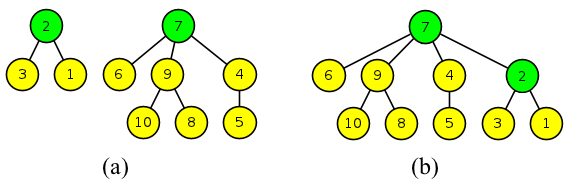
\includegraphics[width=\columnwidth]{obrazky/union.png}
%\caption{\emph{Spájanie podľa ranku.} (a) Pred spojením. (b) Po spojení. 
%Plytší strom sa napojil pod hlbší.} 
%\label{img:union} 
%\end{figure}
\paragraph{Heuristika na spájanie.}

Prvá heuristika pridáva ku algoritmom hodnotu 
$rank(x)$, ktorá bude určovať najväčšiu možnú hĺbku podstromu zakorenenú 
vrcholom $x$. V tom prípade pri o\-pe\-rá\-cií \makeset\ zadefinujeme 
$rank(x) = 0$. 
Pri o\-pe\-rá\-cií \union\ vždy porovnáme $rank(x)$ a $rank(y)$, aby sme zistili, 
ktorý zástupca predstavuje menší strom. Smerník tohto zástupcu potom napojíme 
na zástupcu s výšším rankom. Zástupca novej množiny bude ten s vyšším rankom. 
Ak sú oba ranky rovnaké, vyberieme ľubovoľného zo zástupcov $x$ a $y$, 
jeho rank zvýšime o jeden a smerník ostatného zástupcu bude ukazovať 
na tohto zástupcu. Zástupcom novej množiny bude vybratý zástupca. 

\paragraph{Heuristiky na kompresiu cesty.}

\begin{figure}
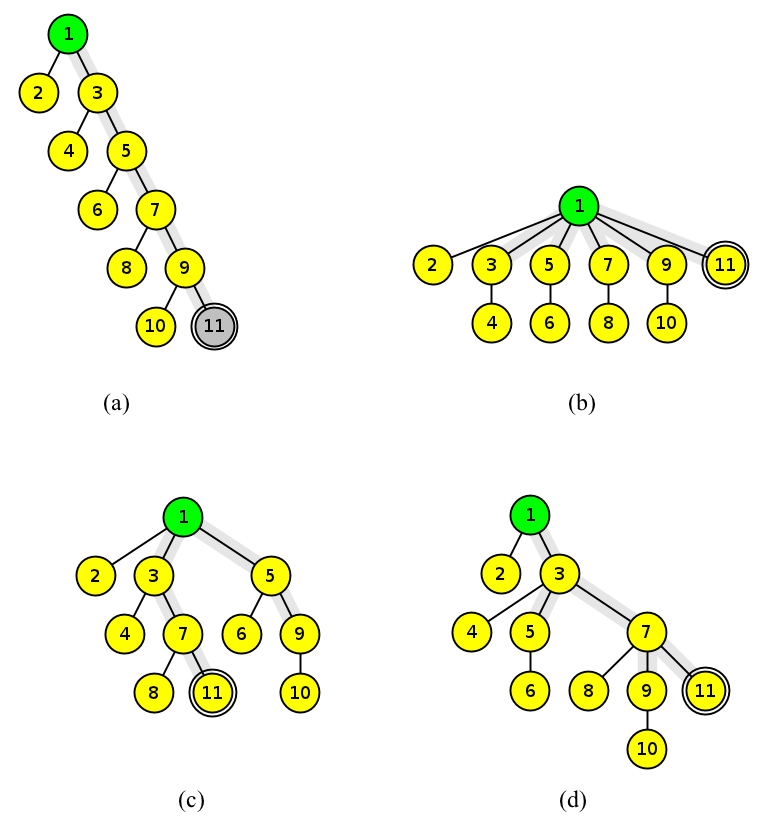
\includegraphics[width=\columnwidth]{obrazky/komp.png}
\caption{\emph{Kompresia cesty z vrcholu 11 do koreňa.} 
Cesta je vyznačená šedou. 
(a) Pred vykonaním kompresie. Pri kompresii~(b) sa všetky vrcholy napoja 
na zástupcu. Pri delení cesty~(c) a pólení cesty~(d) sa cesta skráti 
približne na polovicu.} 
\label{img:komp} 
\end{figure}

Druhou heuristikou je kompresia cesty. Algoritmov na efektívnu kompresiu 
cesty je veľa \citep{paths2}. Tu popíšeme tie najefektívnejšie. Prvou z nich 
je \emph{kompresia} \citep{comp1}. Pri vykonávaní 
operácie \find, po tom, 
ako nájdeme zástupcu množiny obsahujúcej prvok $x$, smerníky prvkov 
navštívených po ceste (vrátane $x$) presmerujeme na zástupcu množiny. Toto 
síce spomalí prvé vykonávanie, ale výrazne zrýchli ďalšie hľadania. 
Druhou heuristikou je \emph{delenie cesty} \citep{comp2}. Pri vykonávaní 
operácie \find\ 
pripojíme každý vrchol\footnote{Okrem koreňa a synov koreňa, 
keďže tie deda a otca resp. deda nemajú.} v ceste od vrcholu $x$ po koreň stromu 
na otca jeho otca. 
Treťou heuristikou je \emph{pólenie cesty} \citep{comp2}. Pri vykonávaní 
operácie \find\ 
pripojíme každý druhý vrchol\footnote{Okrem koreňa a synov koreňa, 
keďže tie deda a otca resp. deda nemajú.} 
v ceste od vrcholu $x$ po koreň stromu na otca jeho otca. 

\bigskip
Časová zložitosť union-findu záleží od toho, koľko prvkov je v množinách a koľko je 
operácií celkovo vykonaných operácií. Všetky uvedené spôsoby ako vykonať 
operáciu \find\ sa dajú použiť s obomi realizáciami operácie \union. 
Počet prvkov označme $n$ a počet operácií $m$. V praxi je zvyčajne počet 
operácií oveľa väčší ako počet prvkov. Pri tomto predpoklade ($m\geq n$) je 
pri použití spájania podľa ranku časová zložitosť pre algoritmus bez kompresie 
$\Theta(m\log n)$ a pre všetky tri uvedené typy kompresií 
$\Theta(m\mathop{\alpha}(m,n))$ \citep{paths2}.

\paragraph{Vizualizácia.} Union-find sme vizualizovali ako les. Pre názorné 
oddelenie množín sme si zvolili pravidlo, ktoré zakazovalo vykresliť vrchol 
napravo od najľavejšieho vrcholu a naľavo od napravejšieho vrcholu inej 
množiny. Jednotlivé množiny sme už vykreslovali tesným Walkerovým algoritmom 
\citep{walker}. 

% V tabuľke~\ref{fig:uf:comp} je porovnanie časových zložitostí \citep{paths2}.

% \begin{table}
% \centering
% \small
% %\footnotesize %toto tu mám nechať?
% \subfloat[Časová zložitosť pre union-find, keď $m \geq n$.][Prehľad časových zložitostí, ak $m \geq n$.]{
% \begin{tabular}{m{2.5cm}m{2.2cm}m{2.2cm}}
% & Naivné spájanie & Spájanie podľa ranku \tabularnewline
% \hline
% Naivné hľadanie & $\Theta\left( mn\right)$ & $\Theta\left( m\log n\right)$ \tabularnewline
% Kompresia, delenie cesty, pólenie cesty & $\Theta\left(m\log _{1+m/n} n \right)$ & $\Theta\left( m\alpha\left( m, n\right) \right)$ \tabularnewline
% \label{fig:uf:comp1}
% \end{tabular}
% }
% \qquad
% \subfloat[Časová zložitosť pre union-find, keď $m < n$.][Prehľad časových zložitostí, ak $m < n$.]{
% \begin{tabular}{m{2.5cm}m{2.2cm}m{2.2cm}}
% & Naivné spájanie & Spájanie podľa ranku \tabularnewline
% \hline
% Naivné hľadanie & $\Theta\left( mn\right)$ & $\Theta\left(n + m\log n\right)$ \tabularnewline
% Kompresia& $\Theta\left(n + m\log  n \right)$ & $\Theta\left(n + m\alpha\left( n, n\right) \right)$ \tabularnewline
% Delenie cesty & $\Theta\left(n \log m \right)$ & $\Theta\left(n + m\alpha\left( n, n\right) \right)$ \tabularnewline
% Pólenie cesty & $\Omega\left(n + m\log n \right)$, $O\left(n\log m\right)$ & $\Theta\left(n + m\alpha\left( n, n\right) \right)$ \tabularnewline
% \label{fig:uf:comp2}
% \end{tabular}}
% \caption{\normalsize Porovnanie časových zložitostí pre rôzne kombinácie hľadaní prvkov a 
% spájaní množín pre union-find. Počet prvkov je $n$ a počet operácií je $m$. $\alpha$ 
% je inverzná Ackermannova funkcia. V praxi zväčša platí, že $m > n$.}
% \label{fig:uf:comp}
% \end{table}

%citovat Walkerov alg. - to mám robiť tu?

